\chapter{Finite Element Approach} \label{cha:FEM_Approach}
Now that we have solved the problem analytically let's go further and introduce a numerical approach, namely \glsfirst{FEM}.
We explain soon both terms \glsfirst{finite} and \glsfirst{element}, but first we need to reformulate the problem.
\section{Weak Formulation}	\label{cha:WeakForm}
Consider again \cref{prb:Normalized_Problem}, i.e.,
\begin{subequations}
	\begin{equation}	\label{eqn:FEM_Problem}
		-\frac{d}{dx} \biggl[ \gls{q} \glsentryname{uPrime} \biggr] = \gls{f}, \quad x \in \left( 0, 1 \right),
	\end{equation}
	with boundary conditions
	\begin{align}
		\gls{u} \bigg \vert_{x = 0} &= \delta,  \label{eqn:FEM_Left_Boundary}  \\
		\biggl[ q \left( x \right) \frac{du}{dx} \biggr]_{x = 1} &= P. \label{eqn:FEM_Right_Boundary}
	\end{align}
\end{subequations}
Now introduce a \gls{r} by
\begin{equation}	\label{eqn:Residual_Function}
	r = \gls{r} = \frac{d}{dx} \left[ \gls{q} \glsentryname{uPrime} \right] + \gls{f} = 0,
\end{equation}
Next multiply both sides of \cref{eqn:Residual_Function} by arbitrary functions
\glsname{wi}\footnote{These are called \glspl{wi} and will be shortly specified.} and integrate the product over
$x \in \left[0, 1\right]$. Thus
\begin{subequations}
	\begin{align}
		\int_{x = 0}^{1} \gls{r} \gls{wi} \dd x &= 0,	\\
		\int_{x = 0}^{1} \frac{d}{dx} \left[ \gls{q} \frac{du}{dx} \right] \gls{wi} \dd x &+
		\int_{x = 0}^{1} \gls{f} \gls{wi} \dd x = 0. \label{eqn:FEM_Rewritten}
	\end{align}
\end{subequations}
%
Applying integration by parts to \cref{eqn:FEM_Rewritten} we get
\begin{equation}  \label{eqn:FEM2_Rewritten}
	\left[ \gls{q} \glsentryname{uPrime} \gls{wi} \right]_{x = 0}^{1}
	- \int_{x = 0}^{1} \gls{q} \frac{ du }{dx} \frac{d \glssymbol{wi}}{dx} \dd x = \int_{x = 0}^{1} \gls{f} \gls{wi} \dd x.
\end{equation}
Since the \gls{normalCondition} is only given on the \gls{rightBoundary}, i.e., at $x = 1$, we choose weight function such that
\begin{equation}
	\gls{wi} \Big \vert_{x = 0 } = 0.  \label{eqn:Weight_Condition}
\end{equation}
Now, insert the \gls{boundaryCondition} and the weight function property, i.e., \cref{eqn:FEM_Right_Boundary,eqn:Weight_Condition},
into \cref{eqn:FEM2_Rewritten} and rearrange the terms,
\begin{equation} \label{eqn:Weak_Formulation}
	\int_{x = 0}^{1} \gls{q} \glsentryname{uPrime} \frac{ d \glssymbol{wi} }{dx} \dd x = P  \gls{wi} \Big \vert_{x = 0} + \int_{x = 0}^{1} \gls{f} \gls{wi} \dd x.
\end{equation}
%
To summarize the \gls{weakForm} we need a couple of definitions. \\
\begin{definition} \label{def:Cont_of_Derivatives}
	Let $n \geq -1$ denote an integer. A general function of a single variable \gls{g} is said to support \gls{ordernCont},
	if and only if the function and its first $n$ derivatives exist and are continuous.
	Integer \glssymbol{orderOfCont} is then called \gls{orderOfCont}.
\end{definition}
Following terminology of \cref{def:Cont_of_Derivatives}, a single-variable function is known as:
\begin{itemize}
	\item discontinuous, if its \gls{orderOfCont} is $\glssymbol{orderOfCont} = -1$.
	\item infinitely differentiable or smooth, if its \gls{orderOfCont} is $\glssymbol{orderOfCont} = \infty$.
		Such a function supports \gls{orderInfCont}.
	\item continuous but not differentiable, if its \gls{orderOfCont} is $\glssymbol{orderOfCont} = 0$.
		Such a function supports \glsentryname{order0Cont}.
	\item up to one-time differentiable, if its \gls{orderOfCont} is $\glssymbol{orderOfCont} = 1$.
		Such a function supports \glsentryname{order1Cont}.
	\item up to two-times differentiable, if its \gls{orderOfCont} is $\glssymbol{orderOfCont} = 2$.
		Such a function supports \glsentryname{order2Cont}, and so on.
\end{itemize}
%
\begin{remark}
	Comparing left hand sides of \cref{eqn:FEM_Rewritten,eqn:Weak_Formulation} we observe that the second derivative involved in
	\cref{eqn:FEM_Rewritten} is replaced by the product of two first derivatives in \cref{eqn:Weak_Formulation}. The original
	requirement of \glsentryname{order1Cont} on \gls{u} is thus replaced by a weaker requirement on \gls{u} and \gls{wi},
	\glsentryname{order0Cont}. This is the reason why \cref{eqn:Weak_Formulation} is called a \gls{weakForm}.
\end{remark}
We conclude that \cref{prb:Normalized_Weak_Problem} below is a \gls{weakForm} of \cref{prb:Normalized_Problem}.
\begin{problem}	\label{prb:Normalized_Weak_Problem}
	Find a function $\gls{u}$ supporting \glsentrysymbol{order0Cont}-continuity such that
	\begin{subequations}
		\begin{align}	\label{eqn:Normalized_Weak_Diff_Eq}
			\int_{x = 0}^{1} \frac{d}{dx} \biggl[ \gls{q} \frac{du}{dx} \biggr] \gls{wi} \dd x
			+\int_{x = 0}^{1} \gls{f} \gls{wi} \dd x &= 0, & x \in \left( 0, 1 \right),
		\end{align}
		with boundary conditions
		\begin{align}
			\gls{u} \bigg \vert_{x = 0} &= \delta,  \label{eqn:Normalized_Weak_Left_Boundary} \\
			\Biggl[ \gls{q} \glsentryname{uPrime} \Biggr]_{x = 1} &= P. \label{eqn:Normalized_Weak_Right_Boundary}
		\end{align}
	\end{subequations}	
\end{problem}

\section[Meshing]{\Gls{meshing}}
Let now \glssymbol{Omega} denote the whole \gls{domain} and divide it into \gls{N} elements
\begin{subequations} \label{eqn:Element_Locations}
	\begin{align}
		\glssymbol{Omega} &= \left[ 0, 1 \right] = \sum \limits_{i = 1}^{\gls{N}} \gls{Omegai}, \label{eqn:Whole_Region}	\\
		\gls{Omegai} &= \left[ \gls{xi},  x_{i + 1}, \right], \quad i = 1, 2, \dots, \gls{N}.	\label{eqn:Element_No_i}
	\end{align}
\end{subequations}
%
This introduces the following concepts:
\begin{definition}
	\Glspl{nodePoint} are distinct and fixed points in the \gls{domain}, i.e.,
	\begin{align}
		x_{i - 1} < & x_{i} < x_{i + 1}, \quad i = 2, 3, \dots, \gls{N}, \\
		x_1  & = 0, \\
		x_{N + 1} & = 1.
	\end{align}
\end{definition}
\begin{definition}
	\Glspl{element} are distinct parts of the \gls{domain}, i.e.,
	\begin{equation}
		\left\{ \glsentryname{Omegae}: \forall x \vert \quad x_{e} \le x \le x_{e + 1}, \quad e = 1, 2, \dots, \gls{N} \right\} .
	\end{equation}
\end{definition}
Note that element boundaries and locations are expressed in \gls{globalCoord}.
\begin{definition}
	\Gls{meshing} is the process of dividing the region into smaller pieces, called elements in FEM terminology. This process
	determines the number of elements, \gls{N}, and the locations of the $N+1$ nodes. Another term for meshing is discretization.
\end{definition}
\begin{remark}
	Two adjacent elements, $\Omega_e$ and $\Omega_{e+1}$, have exactly one common point, $x_{e+1}$.
\end{remark}
\begin{definition}
	A mesh is uniform if all elements have the same size. In the present one-dimensional case, the nodes are therefore equidistant.
\end{definition}
\begin{remark}
	A common procedure is to create an initial mesh, solve the problem, analyze the solution, and then refine or coarsen the mesh
	in regions where the solution varies rapidly or slowly, respectively. This iterative process, \gls{adaptivemeshing}, produces
	a \gls{nonUniformMeshing} and can improve solution accuracy.
\end{remark}
\begin{figure}
	\includegraphics[width = \textwidth]{../Figures/Meshing}
	\caption{A Typical \Gls{region} with \Glspl{element} and \Glspl{nodePoint}}
	\label{fig:Meshing}
\end{figure}
Consider now an approximation to the \gls{exactSol} given by
\begin{equation} \label{eqn:Truncated_FEM_Solution}
	\glssymbol{uM} = \sum_{i = 1}^{\gls{M}} \glsentryname{ai} \gls{phii}.
\end{equation}
This is a series spanned by a total of \gls{M} linearly independent functions \gls{phii}, also called \glspl{shapeFunction} or
\glspl{interpolationFunction}. The series is in addition truncated because we have replaced infinity ($\infty$) on the upper bound of
summation by \gls{M}. The solution in \cref{eqn:Truncated_FEM_Solution} is thus a linear combination of $M$ \glspl{basisFunction}.
and the task is then to determine the \gls{M} coefficients $a_j$, such that \cref{eqn:FEM_Problem}, as well as
\glspl{boundaryCondition} in \cref{eqn:FEM_Left_Boundary,eqn:FEM_Right_Boundary} are satisfied. In FEM-terminology we say that
the model has $M$ \glspl{dof}. \Glspl{basisFunction} have typically \gls{localSupport}, i.e., they are defined over a few \glspl{element}
and are identically $0$ otherwise. \\

The terms \Glsfirst{finite} and \Glsfirstplural{element} in \gls{FEM} refer to the facts that the solution is a truncated series and the
\gls{region} is divided into subregions as explained above. From now on we denote the \gls{FEMSol} just by $u  = u \left( x \right)$
and drop the truncation reference. The first derivative of $u$ may be written as
\begin{equation} \label{eqn:u_Prime}
	\frac{du}{dx} = \sum_{i = 1}^{\gls{M}} a_i \glsentryname{phiiPrime}.
\end{equation}
A particularly interesting choice of weight functions is \glspl{basisFunction}, i.e.,
\begin{subequations} \label{eqn:Weight_Function}
	\begin{align}
		\gls{wi} &= \gls{phii}, & i &= 1, 2, \dots, \gls{M},
		\shortintertext{such that}
		\glsentryname{wiPrime} &= \glsentryname{phiiPrime} & i &= 1, 2, \dots, \gls{M},
	\end{align}
\end{subequations}
Let us for simplicity assume a \gls{uniformMeshing}. Length of all elements is then equal and all nodes are
equidistant Dividing the whole \gls{region} $x \in \left[ 0, 1 \right] $ into \gls{N} \glspl{element} will then result in the
following element locations and element length
\begin{subequations}
	\begin{align}
		\glssymbol{Omega} &= \left[ 0, 1 \right] = \sum \limits_{i = 0}^{\gls{N}} \gls{Omegai}, \\
		\gls{h} & = \frac{x_{N + 1} - x_{1}}{\gls{N}} = \frac{1 - 0}{\gls{N}} = \frac{1}{\gls{N}}.
	\end{align}
	where
	\begin{alignat}{2}
		\gls{Omegai}	&= \left[ \gls{xi},  x_{i + 1} \right], \quad && i = 1, 2, \dots, \gls{N}, \\
		\gls{xi} 		&= \left( i - 1 \right) h, 				\quad && i = 1, 2, \dots, N + 1.
	\end{alignat}
\end{subequations}
 %

The task in this section is to find the \gls{M} unknown coefficients $a_j$. We have to deduce a linear set of equations for coefficients of \glspl{basisFunction},
and then solve it. To do this we begin by \cref{eqn:Weak_Formulation}
\begin{equation*}
	\int_{x = 0}^{1} \gls{q} \frac{du}{dx} \glsentryname{wiPrime} \dd x
		= P \gls{wi} \Big \vert_{x = 1} + \int_{x = 0}^{1} \gls{f}  \gls{wi} \dd x.
\end{equation*}
Insert for $du / dx$ and $dw_i / dx$ from \cref{eqn:u_Prime,eqn:Weight_Function}
\begin{equation}
	\begin{split}
		\int_{x = 0}^{1} \gls{f} \gls{phii} \dd x &+ P \gls{phii} \Big \vert_{x = 1} = \\
		&\quad  \int_{x = 0}^{1} \gls{q} \Biggl[ \sum_{j = 1}^{\gls{M}} a_j
			\frac{ d \varphi_j }{dx} \glsentryname{phiiPrime} \Biggr] \dd x
	\end{split}
\end{equation}
Rearranging the terms we get
\begin{align} \label{eqn:FEM_Eq_Sys}
	\begin{split}
		\sum_{j = 1}^{M} \Biggl[ \int_{x = 0}^{1} \gls{q} \glsentryname{phiiPrime} \glsentryname{phijPrime} \dd x \Biggr] a_j
			&= \int_{x = 0}^{1} \gls{f} \gls{phii} \dd x \\
			& \quad + P \gls{phii} \Big \vert_{x = 1}.
	\end{split}
\end{align}
Define now for $1 \leq i, j \leq M$
\begin{subequations}
	\begin{align}
		\glsentryname{Kij} &= \int_{x = 0}^{1} \gls{q} \glsentryname{phiiPrime} \glsentryname{phijPrime} \dd x,	\label{eqn:Stiffness_Matrix} \\
		\glsentryname{bi} & = P  \gls{phii} \Big \vert_{x = 1} + \int_{x = 0}^{1} \gls{f} \gls{phii} \dd x.	\label{eqn:Load_Vector}
	\end{align}	
\end{subequations}
Note that \cref{eqn:FEM_Eq_Sys} is then a linear system of equations, i.e., 
\begin{subequations}
	\begin{align}	\label{eqn:Compact_Eq_Sys}
		\gls{K} \gls{a} &= \gls{b}, \\
		\sum_{j = 1}^{\gls{M}} \glsentryname{Kij} a_j &= \glsentryname{bi},
	\end{align}
	where
	\begin{alignat}{2}
		\gls{K} &= \left[ \glsentryname{Kij} \right], 	\quad& i,j &= 1, 2, \dots, M, \\
		\gls{a} &= \left[ \glsentryname{ai} \right],	\quad& i   &= 1, 2, \dots, M, \\
		\gls{b} &= \left[ \glsentryname{bi} \right],	\quad& i   &= 1, 2, \dots, M.
	\end{alignat}
\end{subequations}
%
\Gls{basisFunction}s may be chosen among a variety of functions with \gls{globalSupport}
or \gls{localSupport}. It is common, though, to choose them as polynomials with \gls{localSupport}. The polynomial
choice can be defended by the fact that these
functions are easy to evaluate. The \gls{localSupport} means that $\varphi_{i}$ is only non-zero over a few \glspl{element}.
As we will see this gives a sparse banded \gls{stiffnessMatrix}, because basis functions interact only when their supports overlap.
In a \gls{sparseMat}, most entries are zero. In the literature we may find
efficient \glspl{algorithm} for both saving and solving a \gls{linearEquationSystem} with \glspl{sparseMat}. \\

A typical \gls{basisFunction} $\varphi _{i}$ actually consists of two polynomials joined together at \gls{nodePoint} $x_i$.
It would be then desirable that these functions are continuous at the conjuncture. We may also be interested in more
smoothness, for example \glsentryname{order1Cont}. In mathematical formulation we seek \glsname{ordernCont} where $n$ is
a positive integer. While \glsentryname{order0Cont} is achieved by linear polynomials, we have to increase polynomial degree to at
least $3$ to guarantee \glsentryname{order1Cont} and to at least $5$ for \glsentryname{order2Cont}. Both choices of linear and
cubic polynomials for \glspl{basisFunction} are discussed in this report.
%

\section{A Unique Solution}
It is essential to verify if the equation system given in \cref{eqn:Compact_Eq_Sys} has a
\emph{unique} solution. From the linear algebra we know that such a system has always a
unique solution if and only if determinant of the coefficient matrix is nonzero.

\begin{definition} \label{def:Positive_Definite}
	A real square matrix $\gls{matA} \in \gls{Rnn}$ is said to be \gls{posDef} if and only it is symmetrical and
	$\gls{v}^{T} \gls{matA} \gls{v} > 0$, for an arbitrary vector $\gls{v} \in \mathbb{R}^{n \times 1}$
	\begin{subequations}
		\begin{align}
			\gls{matA} &= \gls{matAT}, \label{eqn:Pos_Def_Prop_1} \\
			\gls{v}^{T} \gls{matA} \gls{v} &= \sum \limits_{i = 1}^{n} \sum \limits_{j = 1}^{n} v_{i}  \gls{matAij} v_{j} > 0,
				\quad \forall \mathbf{v} \in \mathbb{R}^{n \times 1} \label{eqn:Pos_Def_Prop_2}
		\end{align}
	\end{subequations}
\end{definition}
\begin{lemma} \label{lem:Pos_Def_Non_Singular}
	Suppose $\gls{matA} \in \gls{Rnn}$ is positive-definite. Then
	\begin{equation}
		\gls{detA} \neq 0.
	\end{equation}
\end{lemma}
For a proof of \cref{lem:Pos_Def_Non_Singular} any textbook in linear algebra may be conferred. In the following we will show
that a \gls{posDef} matrix is \gls{nonSingular} for the simple case of $\mathbf{A} \in \mathbb{R}^{2 \times 2}$. \\
\begin{example}
Suppose that $\gls{matA} \in \glsentryname{R22}$ is a positive-definite matrix given by
\begin{equation}
	\gls{matA} =
	\begin{bmatrix}
		a & b \\
		b & c	
	\end{bmatrix}.
\end{equation}
Then note that
\begin{equation}
\gls{detA} =
	\begin{vmatrix}
		a & b \\
		b & c	
	\end{vmatrix} = a c - b^{2}.
\end{equation}
Now define \gls{v} $\in$ \glsentryname{R21} by
\begin{equation}
	\gls{v} = \begin{bmatrix}	x \\ y	\end{bmatrix},
\end{equation}
and calculate
\begin{equation}	\label{eqn:Temp_Pos_Def_Exp}
	\begin{aligned}
		\gls{v}^T \gls{matA} \gls{v} &=
			\begin{bmatrix} x & y \end{bmatrix}
			\begin{bmatrix} a & b \\ b & c \end{bmatrix}
			\begin{bmatrix} x \\ y \end{bmatrix} \\
		&=	\begin{bmatrix} ax + by & bx + cy \end{bmatrix}
			\begin{bmatrix} x \\ y \end{bmatrix} \\
		&=	ax^{2} + 2bxy + cy^{2}.
	\end{aligned}
\end{equation}
Factoring and rearranging the terms in \cref{eqn:Temp_Pos_Def_Exp} we get
\begin{equation}	\label{eqn:Final_Pos_Def_Exp}
	\begin{aligned}
		\gls{v}^T \gls{matA} \gls{v} &= a \left( x^{2} + \frac{2b}{a} xy + \frac{c}{a} y^{2} \right) \\
		&= a \left( x + \frac{b}{a}y \right)^2 + \frac{c}{a} y^2 - \frac{b^2}{a^2} y^2 \\
		&= a \left( x + \frac{b}{a}y \right)^2 + \frac{ac - b^2}{a^2} y^2 > 0.
	\end{aligned}
\end{equation}
Note that the last inequality is a consequence of the positive-definite property of $\mathbf{A}$. Sufficient
condition to satisfy \cref{eqn:Final_Pos_Def_Exp} is
\begin{equation}
	a > 0, \quad ac - b^2 > 0 \Rightarrow \det(\mathbf{A}) > 0.
\end{equation}
A \gls{posDef} matrix $\mathbf{A}$ $\in \mathbb{R}^{2 \times 2}$ is then non-singular.
\end{example}
\begin{remark}
	A square matrix \gls{matA} $\in$ \gls{Rnn} may be \gls{nonSingular}, $\gls{detA} \neq 0$ without being \gls{posDef}, but
	if the matrix is \gls{posDef} then it is always \gls{nonSingular}, $\gls{detA} \neq 0$. On the other hand, if a matrix
	$\gls{matA}$ is \gls{singular}, it cannot be \gls{posDef}. These statements may be summarized as
	\begin{subequations}
		\begin{align} 
			\gls{matA} \text{ is positive-definite} & \Longrightarrow \gls{detA} \neq 0, \\
			\gls{detA} = 0 & \Longrightarrow \gls{matA} \text{ is not positive-definite}.
		\end{align}
		Thus positive definiteness is a more restrict condition than non-singularity.
	\end{subequations}
\end{remark}

Before imposing the essential boundary condition, the assembled stiffness matrix is only positive semidefinite: the constant function belongs to its nullspace. Uniqueness follows after restricting the discrete space to functions satisfying the homogeneous essential condition at the left boundary.

Let $\mathbf{K}_0$ denote the stiffness matrix on the free degrees of freedom. According to \cref{eqn:Stiffness_Matrix},
\begin{equation}
	\mathbf{K}_0 = \mathbf{K}_0^T.
\end{equation}
For any nonzero free coefficient vector $\mathbf{v}$, let $w_h$ be its associated discrete function. Then $w_h(0)=0$ and
\begin{equation}
	\mathbf{v}^{T}\mathbf{K}_0\mathbf{v}
	= \int_0^1 q(x)\,[w_h'(x)]^2 \dd x > 0. \label{eqn:Pos_Def_Simplified}
\end{equation}
Indeed, equality could hold only if $w_h$ were constant; together with $w_h(0)=0$, this would imply $w_h=0$ and hence $\mathbf{v}=0$. Thus $\mathbf{K}_0$ is positive definite and the constrained Galerkin solution is unique.

The implementation enforces the left value by replacing one matrix row. That full algebraic matrix is nonsymmetric, but it is equivalent to solving the symmetric positive-definite reduced system for the free degrees of freedom.
%

\section{Linear Basis-Functions} \label{cha:Linear_Basis_Function} 
Our first choice of \glspl{basisFunction} are linear polynomials with \gls{localSupport}.
This results in a \gls{FEMSol} supporting \glsentryname{order0Cont}. To span the space of first degree polynomials over an \gls{element}
we need two linearly independent first degree functions. A first degree polynomial needs furthermore two parameters to be fully
specified. We say then a linear polynomial has two degrees of freedom.

\begin{equation} \label{eqn:A_Linear_Polynomial}
	\psi = \psi \left( x \right) = c_0 + c_1 x.
\end{equation}
A \gls{basisFunction} over a single \gls{element} is called a \gls{shapeFunction}. We may use
the two parameters in \cref{eqn:A_Linear_Polynomial} to impose certain values on both end points of the \glspl{shapeFunction}.
Denoting these functions by $\psi_{1}$ and $\psi _{2}$ we may formulate conditions in the \gls{localCoord} as
\begin{subequations} \label{eqn:Cond_On_Linear_Psi_Local}
	\begin{align}
		\psi_{1}\left( 0 \right) & = 1, \label{eqn:Cond_On_Linear_Psi_1_At_Start} \\
		\psi_{1}\left( 1 \right) & = 0, \label{eqn:Cond_On_Linear_Psi_1_At_End} 	\\
		\psi_{2}\left( 0 \right) & = 0, \label{eqn:Cond_On_Linear_Psi_2_At_Start} \\
		\psi_{2}\left( 1 \right) & = 1. \label{eqn:Cond_On_Linear_Psi_2_At_End}
	\end{align}
\end{subequations}
Next we insert conditions in \crefrange{eqn:Cond_On_Linear_Psi_1_At_Start}{eqn:Cond_On_Linear_Psi_2_At_End}
into \cref{eqn:A_Linear_Polynomial}. For each \gls{shapeFunction} we then get two equations with two unknowns, $c_0$ and $c_1$.
Solving these systems give fully specified \glspl{shapeFunction} as 
\begin{subequations}	\label{eqn:Linear_Psi_Local}
	\begin{align}
		\psi_{1} \left( x \right) &= 1 - x, \\
		\psi_{2} \left( x \right) &= x.
	\end{align}
\end{subequations}
\begin{figure}
	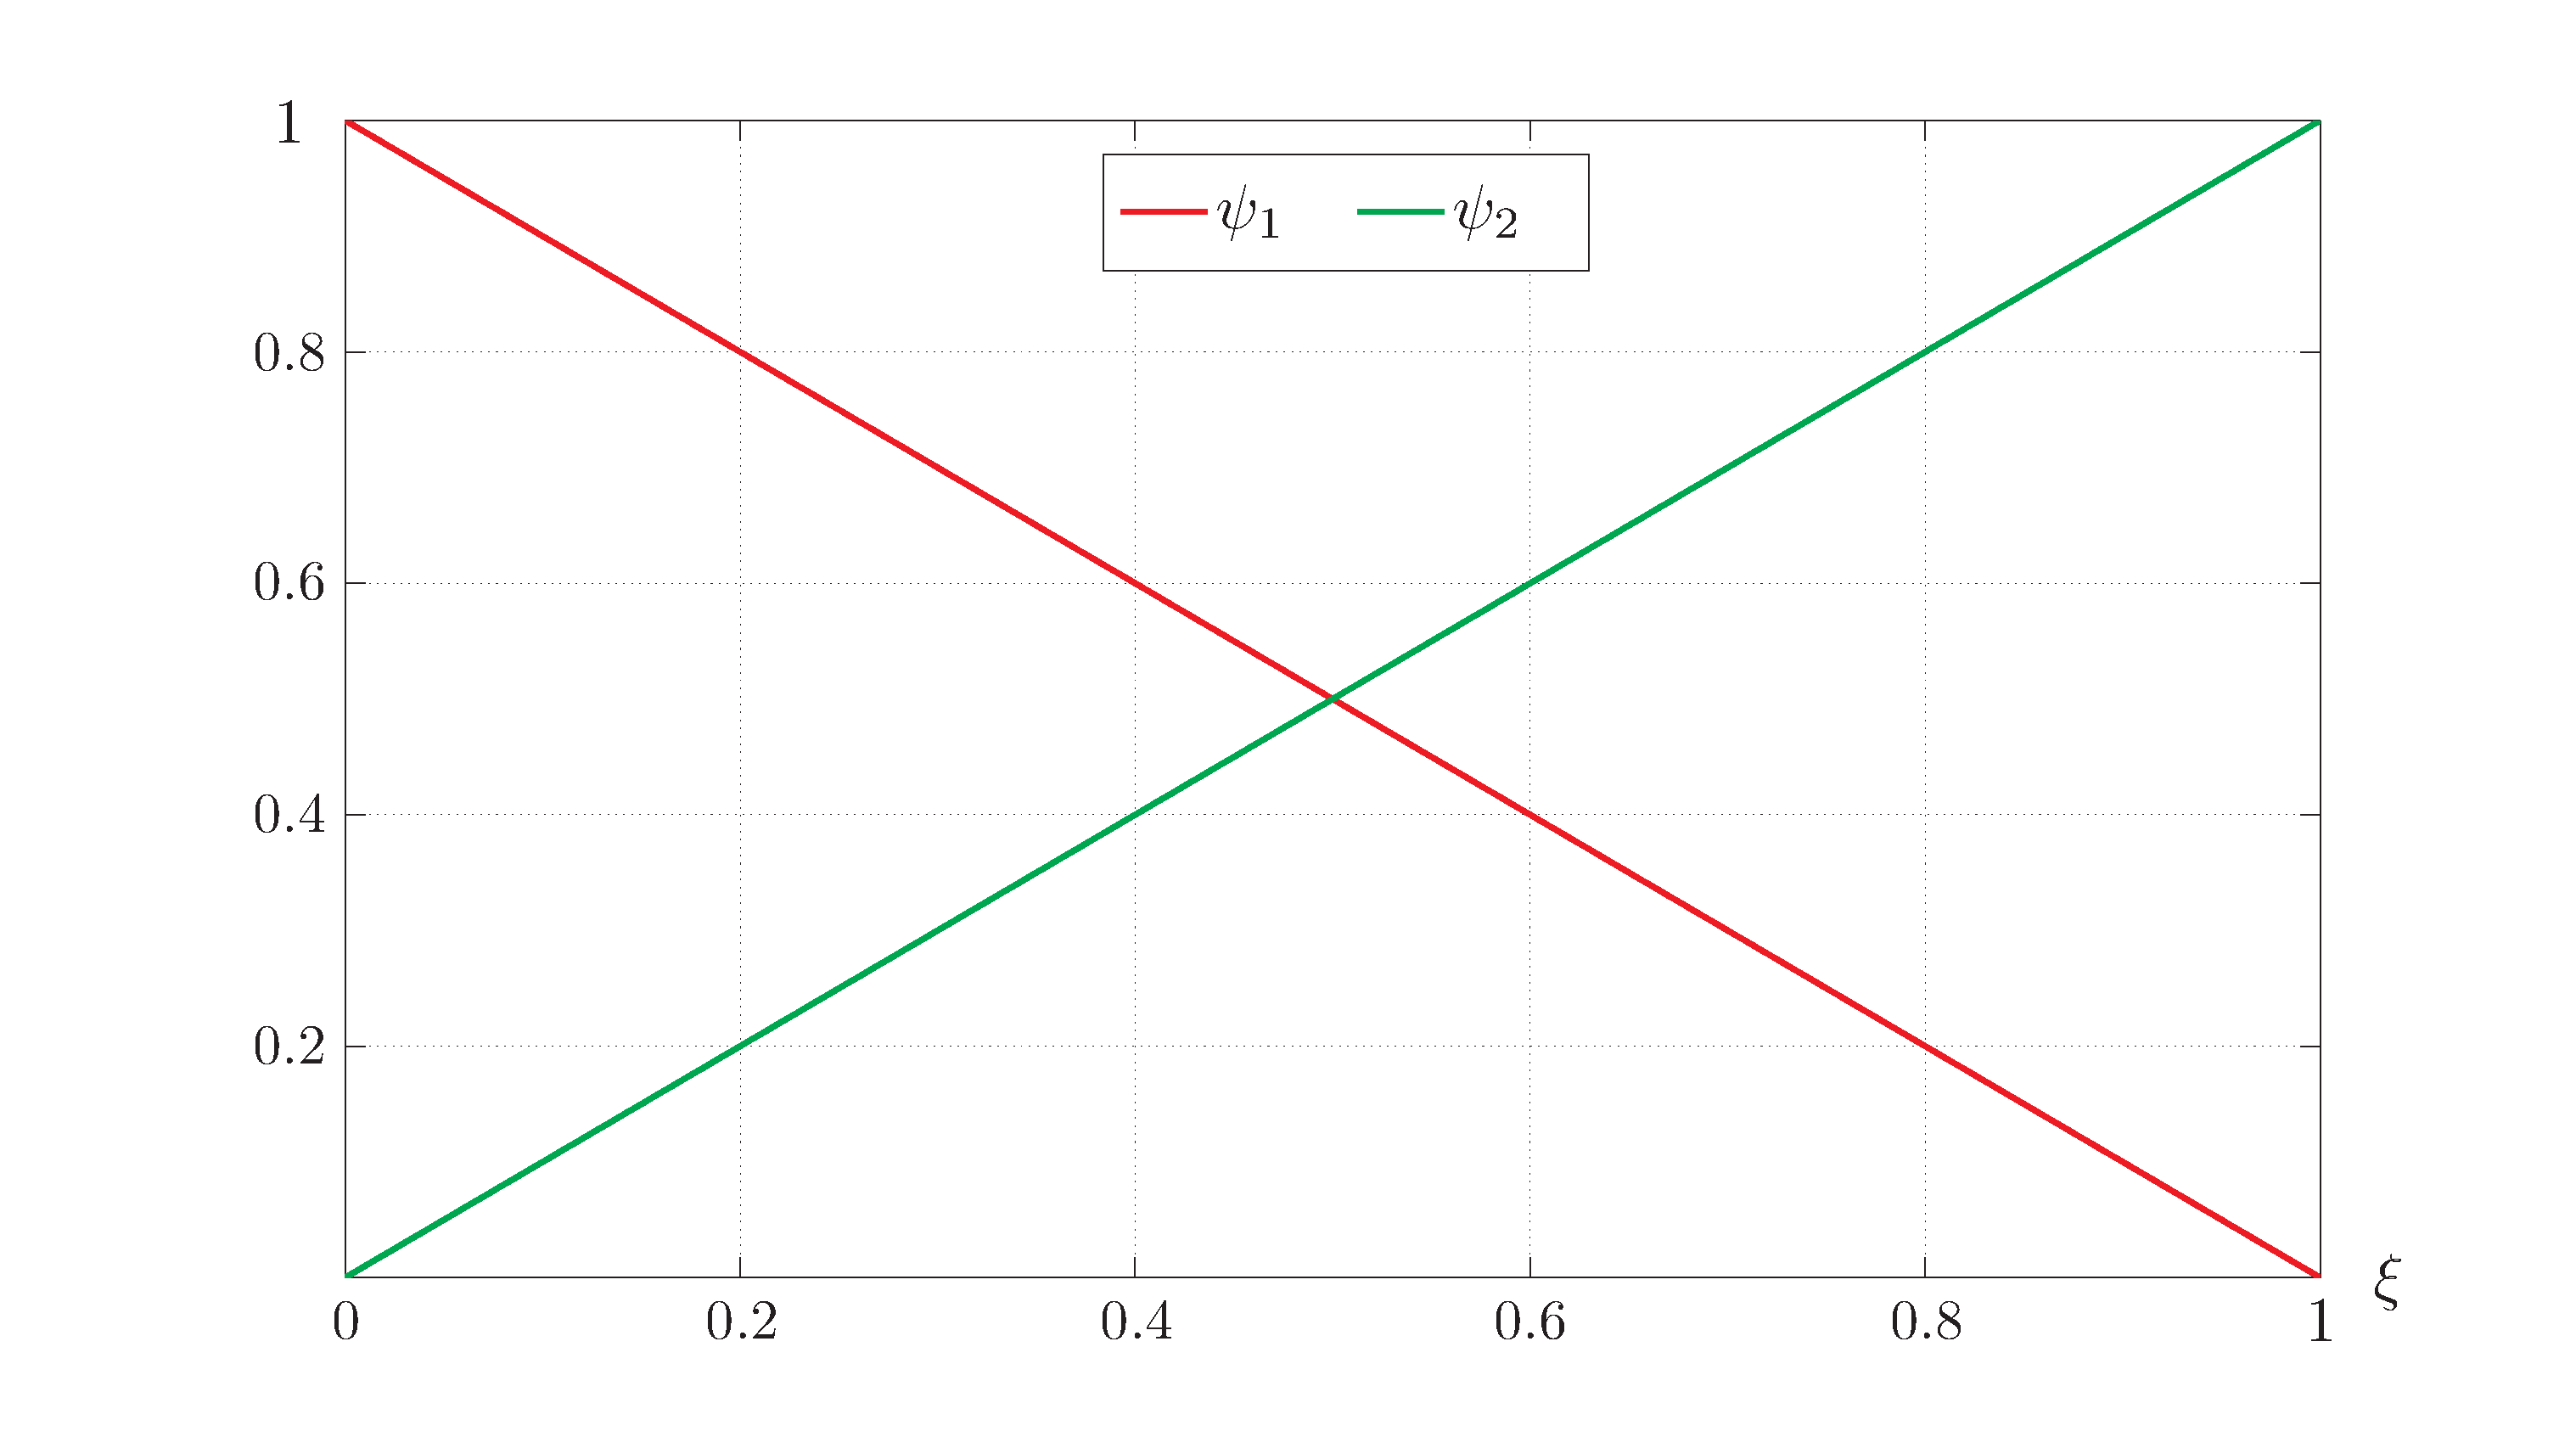
\includegraphics[width = \textwidth]{../figures/linear-shape-functions}
	\caption[Choice of Linear Polynomials for Shape Functions]{Choice of Linear Polynomials for Shape Functions}
	\label{fig:Linear_Shape_Functions}
\end{figure}
\begin{figure}
	
\includegraphics[width = \textwidth]{../Figures/linear-basis-functions}
	\caption[Choice of Cubic Polynomials for Basis-Functions]
		{Choice of linear polynomials for Basis-Functions gives a solution which is $\mathcal{O} \left( 0 \right)$-continuous.}
		\label{fig:Linear_Basis_Functions}
\end{figure}
The linear \glspl{shapeFunction} and \gls{piecewiseLinear} polynomials over the whole \gls{region} are shown in
\cref{fig:Linear_Shape_Functions,fig:Linear_Basis_Functions}, respectively. Observe that a \gls{basisFunction} $\varphi _{i}\left( x\right)$
consists of two \glspl{shapeFunction} joined at \gls{nodePoint} $x_{i}$. \Glspl{basisFunction} are therefore \gls{piecewiseLinear} polynomials.
We see clearly that \glspl{basisFunction} support \glsentryname{order0Cont}. Thus for $i = 2, 3, \dots, N$
\begin{subequations} \label{eqn:Phi_i_Linear}
	\begin{align}
		\varphi_{i} \left( x_{i-1} \right) & = 0,  \label{eqn:Phi_i_At_Left_End} \\
		\lim_{x \rightarrow x_{i}^{-}} \varphi_{i} \left( x \right) & =
		\lim_{x \rightarrow x_{i}^{+}} \varphi_{i} \left( x \right) = 1,	\label{eqn:Phi_i_At_Center} \\
		\varphi_{i}\left( x_{i + 1} \right) & = 0.  \label{eqn:Phi_i_At_Right_End}
	\end{align}
\end{subequations}
Conjuncture is irrelevant for the first and last \glspl{basisFunction}, due to the fact that they are only defined over one element. Thus
\begin{subequations} \label{eqn:Phi_Boundaries}
	\begin{align}
		\varphi_{1} \left( x_{1} \right) & = 1,  \label{eqn:Phi_1_At_x_1} \\
		\varphi_{1} \left( x_{2} \right) & = 0,  \label{eqn:Phi_1_At_x_2} \\
		\varphi_{N + 1} \left( x_{N} \right) & = 0,  \label{eqn:Phi_N_Plus_1_At_x_N} \\
		\varphi_{N + 1} \left( x_{N + 1} \right) & = 1.  \label{eqn:Phi_N_Plus_1_At_x_N_Plus_1}
	\end{align}
\end{subequations}
\Gls{nodePoint} $x_{i}$ where $\varphi _{i}$ takes on the unity value is called the home node of $\varphi _{i}$. The node point
$x_{i}$ is also the joint point between two pieces of linear polynomials and thus the condition in \cref{eqn:Phi_i_At_Center}
guarantees \glsentryname{order0Cont}. Furthermore, for $j = 1, 2, \dots, N$, \cref{eqn:Phi_i_Linear} results in
\begin{equation} \label{eqn:u_At_x_j}
	\begin{aligned}
		\glsentryname{uAtXj} & = \sum_{i = 1}^{N + 1} \glsentryname{ai} \glsname{phii} \Big \vert_{x = x_j} \\
		& = a_j \varphi_{j} \left( x_j \right) \\
		& = a_j.
	\end{aligned}
\end{equation}
As we see later we can use \cref{eqn:u_At_x_j} to implement the Dirichlet condition on the left boundary.
%
\subsection[Element Matrix]{\Gls{elementMatrix}} \label{cha:Element_Matrix_Linear}
The global integral involved in calculation of the \gls{stiffnessMatrix} in \cref{eqn:Stiffness_Matrix} may be written as a sum of
integrals each over a single \gls{element}, i.e., 
\begin{equation} \label{eqn:Stiffness_Entries_Linear_1}
	\begin{aligned}
			\glsentryname{Kij} &= \int_{x = 0}^{1} \gls{q} \glsentryname{phiiPrime} \glsentryname{phijPrime} \dd x \\
			&= \sum \limits_{e = 1}^{\gls{N}} \int_{x \in \Omega_{e}} \gls{q} \glsentryname{phiiPrime} \glsentryname{phijPrime} \dd x.
	\end{aligned}
\end{equation}
Observe that $\varphi_i \left( x \right)$ is only non-zero over the two \gls{adjacentElements} $\Omega_{i - 1}$ and $\Omega_{i}$.
In the same manner $\varphi_j \left( x \right)$ is only non-zero over $\Omega_{j - 1}$ and $\Omega_{j}$. Thus the global stiffness
matrix is tridiagonal, i.e.,
\begin{equation}	\label{eqn:Global_Stiffness_Properties}
	\begin{aligned}
			\gls{Kij}	&= K_{j,i} \neq 0, 	&&	j = i - 1,  i,  i + 1, \\
			\gls{Kij}	&= K_{j,i} = 0, 	&&	\text{otherwise.}
	\end{aligned}
\end{equation}
\Cref{eqn:Stiffness_Entries_Linear_1} is then reduced to
\begin{subequations}	\label{eqn:Stiffness_Linear}
	\begin{align}
		\glsentryname{Kij} &= \int_{ x_{i - 1} }^{ x_{i} } \gls{q} \glsentryname{phiiPrime} \glsentryname{phijPrime} \dd x
		+\int_{ x_{i} }^{ x_{i + 1} } \gls{q} \glsentryname{phiiPrime} \glsentryname{phijPrime} \dd x.
		\label{eqn:Stiffness_Entries_Linear}
	\end{align}
	Thus
	\begin{align}
		K_{i, i} &= \int_{ x_{i - 1} }^{ x_{i} } \gls{q} \bigg( \glsentryname{phiiPrime} \bigg)^2 \dd x
				+\int_{ x_{i} }^{ x_{i + 1} } \gls{q} \bigg( \glsentryname{phiiPrime} \bigg)^2 \dd x
			\label{eqn:Stiffness_Linear_Diag0_1} \\
		K_{i, i + 1} &= K_{i + 1, i} = \int_{ x_{i} }^{ x_{i + 1} } \gls{q} \frac{ d \varphi_i }{ dx } \frac{ d \varphi_{i + 1} }{ dx } \dd x.
			\label{eqn:Stiffness_Linear_Diag1_1}
	\end{align}
\end{subequations}
Consider now \cref{eqn:Stiffness_Linear_Diag1_1} and note that it consists of contribution from a single element,
$\Omega_{i}$. We have derived shape functions in terms of the local variable $\xi \in \left[ 0, 1 \right]$. Generally speaking,
we need then a transformation from the global variable $x \in \Omega_{e} = \left[ x_e, x_{e + 1} \right]$ to the local variable
$\xi \in \left[ 0, 1 \right]$. This brings the global basis-function $\varphi_i$ back to the local shape functions
$\psi_m, \quad m = 1, 2$. The variable change is given by
\begin{equation}	\label{eqn:Global_2_Local_1}
	\begin{alignedat}{3}
		\xi	  &= \frac{x-x_{e}}{x_{e+1}-x_{e}}	\quad& \Leftrightarrow \quad&& x  &= x_{e}+\left(x_{e+1}-x_{e} \right) \xi, \\
		d \xi &= \frac{1}{x_{e + 1} - x_{e}} dx	\quad& \Leftrightarrow \quad&& dx &= \left(x_{e+1}-x_{e} \right) d \xi.
	\end{alignedat}
\end{equation}
Assuming a uniform discretization the change of variable is simplified to
\begin{equation}	\label{eqn:Global_2_Local}
	\begin{alignedat}{3}
		\xi		&= 1 - e + \frac{1}{h} \quad& \Leftrightarrow \quad&&	x  &= \left( e - 1 + \xi \right) h,	\\
		d \xi	&= \frac{1}{h} dx \quad& \Leftrightarrow \quad&&		dx &= hd \xi.
	\end{alignedat}
\end{equation}
Now apply the transformation in \cref{eqn:Global_2_Local} with $e = i$ to \cref{eqn:Stiffness_Linear_Diag1_1}. Then
\begin{subequations}
	\begin{align}
		K_{i, i + 1} &= K_{i + 1, i} = \int_{ ih }^{ \left( i + 1 \right) h } \gls{q} \frac{ d \varphi_i }{ dx }
			\frac{ d \varphi_{i + 1} }{ dx } \dd x	\label{eqn:Element_Stiffness_Entries_1} \\
		&= \int_{ 0 }^{ 1 } q \Bigl[ \left( i - 1 + \xi \right) h \Bigr] \frac{ d \psi_1 }{ d \xi } \frac{d \xi}{ dx }
			\frac{ d \psi_2 }{ d \xi } \frac{ d \xi }{dx} \dd \xi.	\label{eqn:Element_Stiffness_Entries_2} 
	\end{align}
\end{subequations}
Note that \cref{eqn:Element_Stiffness_Entries_1} is deduced from \cref{eqn:Element_Stiffness_Entries_2} by applying Chain Rule to 
$\frac{ d \varphi_i }{ dx }$ and $\frac{ d \varphi_{i + 1} }{ dx }$. Some simplification gives
\begin{align}
		K_{i, i + 1} &= K_{i + 1, i} = \frac{1}{h} \int_{0}^{1} q \Bigl[ \left( i - 1 + \xi \right) h \Bigr] \frac{ d \psi_1 }{ d \xi } \frac{ d \psi_2 }{ d \xi } \dd \xi.
\end{align}
Applying variable transformation in \cref{eqn:Global_2_Local} with $e = i - 1$ and $e = i$ to \cref{eqn:Stiffness_Linear_Diag0_1} 
we get
\begin{equation}
	\begin{split}
		K_{i, i} &= \frac{1}{h} \int_{0}^{1} q \Bigl[ \left( i - 2 + \xi \right) h \Bigr]
			\biggl( \frac{ d \psi_1 }{ d \xi } \biggr)^2 \dd \xi	\\
		&\quad + \frac{1}{h} \int_{0}^{1} q \Bigl[ \left( i - 1 + \xi \right) h \Bigr]
			\biggl( \frac{ d \psi_2 }{ d \xi } \biggr)^2 \dd \xi.
	\end{split}
\end{equation}
Calculation of \gls{Kij} is then summarized by
\begin{subequations}
	\begin{equation}
		\begin{aligned}
			\gls{Kij}	&= K_{22}^{i - 1} + K_{11}^{i},	&& j = i,	\\
			\gls{Kij}	&= K_{j,i} = K_{1,2}^i,			&& j = i - 1, i + 1,	\\
			\gls{Kij}	&= 0,							&& otherwise,
		\end{aligned}
	\end{equation}
	where \glsentryname{Kmne} represents contribution of element No. $e$ to the global stiffness matrix given by
	\begin{equation}	\label{eqn:Element_Stiffness_Entries_3}
		\glsentryname{Kmne} = \int_{0}^{1} q \Bigl[ \left( e - 1 + \xi \right) h \Bigr]
			\frac{ d \psi_m }{ d \xi } \frac{ d \psi_n }{ d \xi } \dd \xi,	\quad m, n = 1, 2.
	\end{equation}
\end{subequations}
%
\subsection[Element Load]{\Gls{elementLoad}} \label{cha:Element_Load_Linear}
Summation over all \glspl{element} may also be carried out under calculation of the global \gls{loadVector}. For simplicity we repeat load vector
components from \cref{eqn:Load_Vector}
\begin{equation}
	\glsentryname{bi} = P  \varphi _{i}\left( x \right) \Bigg \vert_{x = 1} +
	\int_{0}^{1} \gls{f} \gls{phii} \dd x.
\end{equation}
Note again that the only non-zero basis-function at $x = 1$ is the last one, i.e.,
\begin{align}
	\varphi_i \left( x \right) \Big \vert_{x = 1} &= 
	\begin{cases}
		0,	& i = 1, 2, \dots, N,	\\
		1,	& i = N + 1.
	\end{cases}
\end{align}
Then load entries are given by
\begin{subequations}	\label{eqn:Linear_Load_Components}
	\begin{align}
		b_{i} &= \int_{0}^{1} \gls{f} \gls{phii} \dd x - \int_{0}^{1} \gls{q} \glsentryname{thetaPrime} \dd x,
			\quad 1 \leq i \leq \gls{N}, \label{eqn:Typical_Load_Component} \\
		b_{N + 1} &= P + \int_{0}^{1} \gls{f} \varphi_{N + 1} \left( x \right) \dd x.	\label{eqn:Last_Load_Component} 
	\end{align}
\end{subequations}
Now applying variable transformation in \cref{eqn:Global_2_Local} to a typical load element in \cref{eqn:Typical_Load_Component} gives
\begin{equation} \label{eqn:Load_Summation}
		\glsentryname{bi}	= h \int_{ 0 }^{ 1 } f \Bigl[ \left( i - 2 + \xi \right) h \Bigr] \psi_2 \left( \xi \right)
			+ h \int_{ 0 }^{ 1 } f \Bigl[ \left( i - 1 + \xi \right) h \Bigr] \psi_1 \left( \xi \right).
\end{equation}
We will look at the first and last entry of load vector shortly. A typical global load element is given by
\begin{subequations}
	\begin{equation}
		b_{i} = b_{2}^{i - 1} + b_{1}^{i},	\quad i = 2, ... N,
	\end{equation}
	where
	\begin{equation}
		\begin{split}
			b_{m}^{e} &= h \int_{ 0 }^{ 1 } f \Bigl[ \left( e - 1 + \xi \right) h \Bigr] \psi_m \left( \xi \right)	\\
			&\quad -h \int_{0}^{1} q \Bigl[ \left(e-1+\xi \right) h \Bigr] \glsentryname{thetaPrime} \dd \xi, \quad m = 1,2.	
		\end{split}
	\end{equation}
\end{subequations}
%
\subsection{Assembly Process} \label{cha:Assembly_Process_Linear}
We have seen how to construct \glspl{elementMatrix} and \glspl{elementLoad}. \emph{\Gls{assembly}}
is a process where we go through all \glspl{element} and add each element's contribution, i.e., \gls{elementMatrix} and
\gls{elementLoad}, to the global \gls{stiffnessMatrix} and \gls{loadVector}. \\

Now, denote by $\gls{K}$ and $\gls{b}$ the global \gls{stiffnessMatrix} and the global \gls{loadVector}.
Furthermore, let \gls{KGlobalE} and \gls{bGlobalE} denote the global \gls{stiffnessMatrix} and the global \gls{loadVector}
after contributions from elements $1, 2, \dots, e$ are added. Thus $\gls{K} = \mathbf{K}^{ \left( N \right) }$ and
$b = \mathbf{b}^{\left( N \right)}$. Then in a \gls{region} with $N = 4$ \glspl{element}, the global
stiffness matrix and load vector is constructed by a stepwise process sketched in
\crefrange{fig:K_1_Linear}{fig:K_4_Linear} and \cref{fig:b_1_To_b_4_Linear}, respectively.
%
% --------------- Insert Visualization of Linear Assembly Process --------------
% Linear K^{1}
\begin{figure}[H]
	\centering
	\begin{equation*}
		\mathbf{K}^{\left( 1 \right)} =
		\begin{bmatrix}
			k_{11}^{1} & k_{12}^{1} & 0 & 0 & 0 \\ \\
			k_{21}^{1} & k_{22}^{1} & 0 & 0 & 0 \\ \\
			0 & 0 & 0 & 0 & 0 \\ \\
			0 & 0 & 0 & 0 & 0 \\ \\
			0 & 0 & 0 & 0 & 0
		\end{bmatrix}
	\end{equation*}
	\caption{Stiffness Assembly with Linear Basis-Functions, $\mathbf{K}^{\left(1\right)}$ }
	\label{fig:K_1_Linear}
\end{figure}
% Linear K^{2}
\begin{figure}[H]
	\centering
	\begin{equation*}
		\mathbf{K}^{\left( 2 \right)} =
		\begin{bmatrix}
			k_{11}^{1} & k_{12}^{1} & 0 & 0 & 0 \\ \\
			k_{21}^{1} & k_{22}^{1} + k_{11}^{2} & k_{12}^{2} & 0 & 0 \\ \\
			0 & k_{21}^{2} & k_{22}^{2}	& 0 & 0 \\ \\
			0 & 0 & 0 & 0 & 0 \\ \\
			0 & 0 & 0 & 0 & 0
		\end{bmatrix}
	\end{equation*}
	\caption{Stiffness Assembly with Linear Basis-Functions, $\mathbf{K}^{\left(2\right)}$ }
	\label{fig:K_2_Linear}
\end{figure}
%
% Linear K^{3}
\begin{figure}[H]
	\centering
	\begin{equation*}
		\mathbf{K}^{\left( 3 \right)} =
		\begin{bmatrix}
			k_{11}^{1} & k_{12}^{1} & 0 & 0 & 0 \\ \\
			k_{21}^{1} & k_{22}^{1} + k_{11}^{2} & k_{12}^{2} & 0 & 0 \\ \\
			0 & k_{21}^{2} & k_{22}^{2} + k_{11}^{3} & k_{12}^{3} & 0 \\ \\
			0 & 0 & k_{21}^{3} & k_{22}^{3}	& 0 \\ \\
			0 & 0 & 0 & 0 & 0
		\end{bmatrix}
	\end{equation*}
	\caption{Stiffness Assembly with Linear Basis-Functions, $\mathbf{K}^{\left(3\right)}$ }
	\label{fig:K_3_Linear}
\end{figure}
%
% Linear K^{4}
\begin{figure}[H]
	\centering
	\begin{equation*}
		\mathbf{K}^{\left( 4 \right)} =
		\begin{bmatrix}
			k_{11}^{1} & k_{12}^{1} & 0 & 0 & 0 \\ \\
			k_{21}^{1} & k_{22}^{1} + k_{11}^{2} & k_{12}^{2} & 0 & 0 \\ \\
			0 & k_{21}^{2} & k_{22}^{2} + k_{11}^{3} & k_{12}^{3} & 0 \\ \\
			0 & 0 & k_{21}^{3} & k_{22}^{3} + k_{11}^{4} & k_{12}^{4} \\ \\
			0 & 0 & 0 & k_{21}^{4} & k_{22}^{4}
		\end{bmatrix}
	\end{equation*}
	\caption{Stiffness Assembly with Linear Basis-Functions, $\mathbf{K}^{\left(4\right)}$ }
	\label{fig:K_4_Linear}
\end{figure}
%
% Linear Load b^{1}, ... , b^{4}
\begin{figure}[H]
	\centering
	% b_{1}
	\begin{align*}
	\mathbf{b}^{\left( 1 \right)} &=
	\begin{bmatrix}
	b_{1}^{1} & b_{2}^{1} & 0 & 0 & 0
	\end{bmatrix}^{T},	\\
	% b_{2}
	\mathbf{b}^{\left( 2 \right)} &=
	\begin{bmatrix}
	b_{1}^{1} & b_{2}^{1} + b_{1}^{2} & b_{2}^{2} & 0 & 0
	\end{bmatrix}^{T},	\\
	% b_{3}
	\mathbf{b}^{\left( 3 \right)} &=
	\begin{bmatrix}
	b_{1}^{1} & b_{2}^{1} + b_{1}^{2} & b_{2}^{2} + b_{1}^{3} & b_{2}^{3} & 0
	\end{bmatrix}^{T},	\\
	% b_{4}
	\mathbf{b}^{\left( 4 \right)} &=
	\begin{bmatrix}
	b_{1}^{1} & b_{2}^{1} + b_{1}^{2} & b_{2}^{2} + b_{1}^{3} & b_{2}^{3} + b_{1}^{4} & b_{2}^{4}
	\end{bmatrix}^{T}.
	\end{align*}
	\caption{Load Assembly with Linear Basis-Functions, $\mathbf{b}^{\left( 1 \right)}, \dots, \mathbf{b}^{ \left( 4 \right) }$}
	\label{fig:b_1_To_b_4_Linear}
\end{figure}
%

%
\section{Cubic Basis-Functions} \label{cha:Cubic_Basis_Function}
Cubic polynomial basis functions are widely used in FEM, including in one-dimensional problems.
There are several reasons for this popularity:
\begin{enumerate}
	\item Cubic basis functions support \glsentryname{order1Cont}, producing a smoother solution than the linear choice.

	\item They generally provide a more accurate solution and a higher convergence rate than the linear case.

	\item The additional cost of using cubic rather than linear basis functions is modest, especially in one dimension.
\end{enumerate}
%
In the linear case, one basis function was associated with each node, giving $N+1$ functions and two shape functions per element.

In the cubic case, on the other hand, we need $4$ \glspl{shapeFunction} over each \gls{element}, or totally $2N + 2$ \glspl{basisFunction}.
Each cubic \gls{shapeFunction} has 4 parameters and thus must have $4$ conditions to be fully specified. The first $2$ conditions
concern function values at the \glspl{nodePoint}, while the last $2$ give values of first derivatives at the same node points. \\

The first \gls{shapeFunction} $\psi_1$, guarantees function values $1$ and $0$ on the left and right element boundaries, as well as a
vanishing derivative at both ends
\begin{subequations}	\label{eqn:Cond_On_Cubic_Psi_1_Local}
	{\allowdisplaybreaks
		\begin{align}
			\psi_{1} \left( 0\right) &= 1,	\\
			\psi_{1} \left( 1 \right) &= 0,	\\
			\psi_{1,  x}\left( 0 \right) &= 0,	\\
			\psi_{1,  x}\left( 1 \right) &= 0.
		\end{align}
	}% end of \allowdisplaybreaks
\end{subequations}
The second \gls{shapeFunction} has a value of unity at the right boundary, otherwise function and derivative values of zero at the boundaries.
In the same manner the third and fourth \glspl{shapeFunction} have their unity values for the derivative at the left and right boundaries.	\\

A general cubic polynomial and its derivative may be written as
\begin{subequations}
	\begin{align}
		\psi _{i}\left( x \right) &= c_{0} + c_{1} x + c_{2}x^{2} + c_{3}x^{3},	\label{eqn:General_Cubic_Func}	\\
		\psi _{i}^{\prime} \left( x \right) &= c_{1} + 2c_{2}x + 3c_{3}x^{2}.	\label{eqn:General_Cubic_Der}
	\end{align}
\end{subequations}
%
For each \gls{shapeFunction} coefficients $c_1, \dots, c_4$ may be found by applying conditions above to
\cref{eqn:General_Cubic_Func,eqn:General_Cubic_Der}. Here are the results
\begin{subequations}	\label{eqn:Cubic_Psi_Local}
	\begin{align}
		\psi _{1}\left( x \right) &= 1 - 3 x^{2} + 2x^{3},	\\
		\psi _{2}\left( x \right) &= 3 x^{2} - 2 x^{3},	\\
		\psi _{3}\left( x \right) &= x - 2 x^{2} + x^{3},	\\
		\psi _{4}\left( x \right) &= -x^{2} + x^{3}.
	\end{align}
\end{subequations}
%
Cubic \glspl{shapeFunction} and \gls{piecewiseCubic}
polynomials over the whole domain are depicted in \cref{fig:Cubic_Shape_Functions,fig:Cubic_Basis_Functions}, respectively. Observe
from the latter that the first $N+1$ functions control the solution value at \glspl{nodePoint}, while the last $N+1$ functions
take care of first derivatives at \glspl{nodePoint}. \\	\\
Thus using \cref{eqn:Truncated_FEM_Solution} with $M = 2N + 2$, the solution value at \glspl{nodePoint} may be written as
\begin{subequations}
	\begin{align}
		% Function u(x)
		\gls{u} &= \sum_{i = 1}^{2N + 2} \glsentryname{ai} \gls{phii},	\notag \\
		% Function value at x = x_j
		\glsentryname{uAtXj} &= \sum_{i = 1}^{2N + 2} \glsentryname{ai} \gls{phii} \bigg \vert_{x = x_j} = a_j,	\label{eqn:Cubic_Solution_At_X_i}
	\end{align}
	In the same manner we apply \cref{eqn:u_Prime} with $M = 2N + 2$ to find the first derivative values at the \glspl{nodePoint}, i.e.,
	\begin{equation}
		% First derivate at x_j,
		\glsentryname{uPrimeAtXj} = \sum_{i = 1}^{2N + 2} a_i \glsentryname{phiiPrime} \bigg \vert_{x = x_j}
		= a_{j + N + 1}.	\label{eqn:Cubic_Solution_Derivative_At_X_i}
	\end{equation}
\end{subequations}
%
Thus the cubic choice results in $M = 2N + 2$ \glspl{dof}. \Glspl{shapeFunction} and their derivatives, in both the linear and
cubic case are implemented in \cref{lst:Def_FEM_Func}.
\begin{figure}
	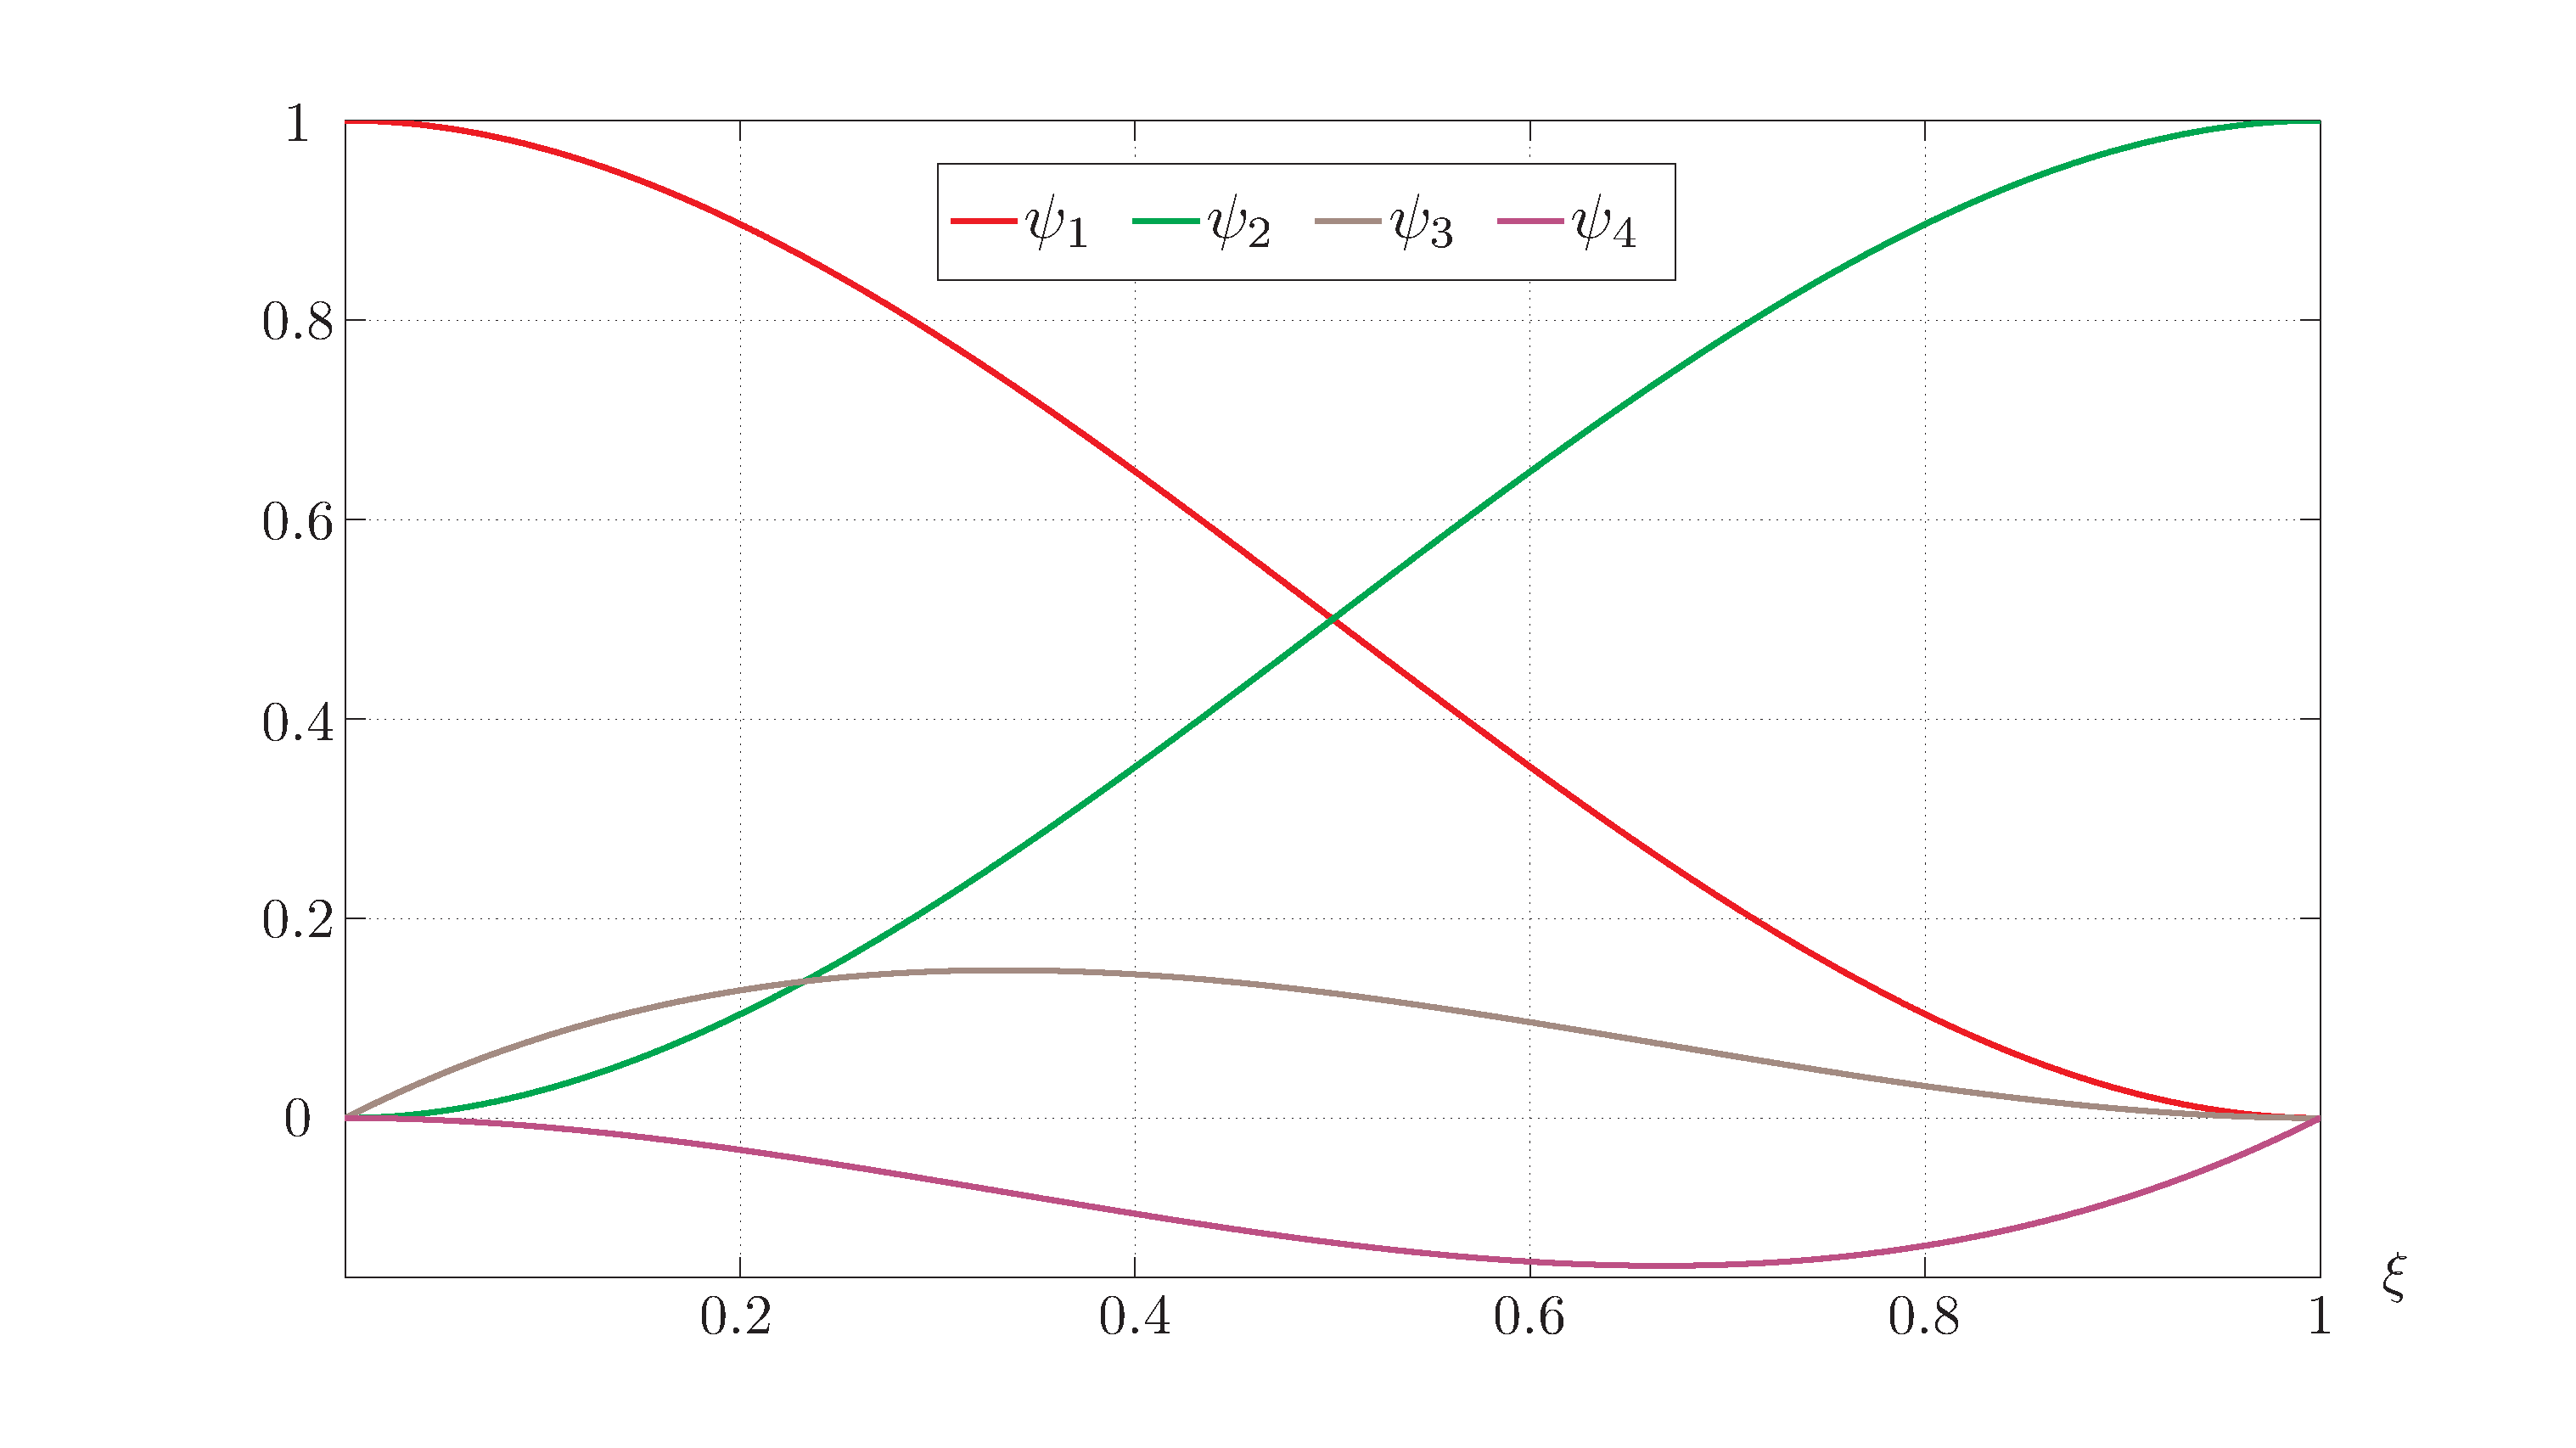
\includegraphics[width = \textwidth]{../figures/cubic-shape-functions}
	\caption[Choice of Cubic Polynomials for Shape-Functions]
		{Choice of Cubic Polynomials for Shape-Functions}
	\label{fig:Cubic_Shape_Functions}
\end{figure}
\begin{figure}
	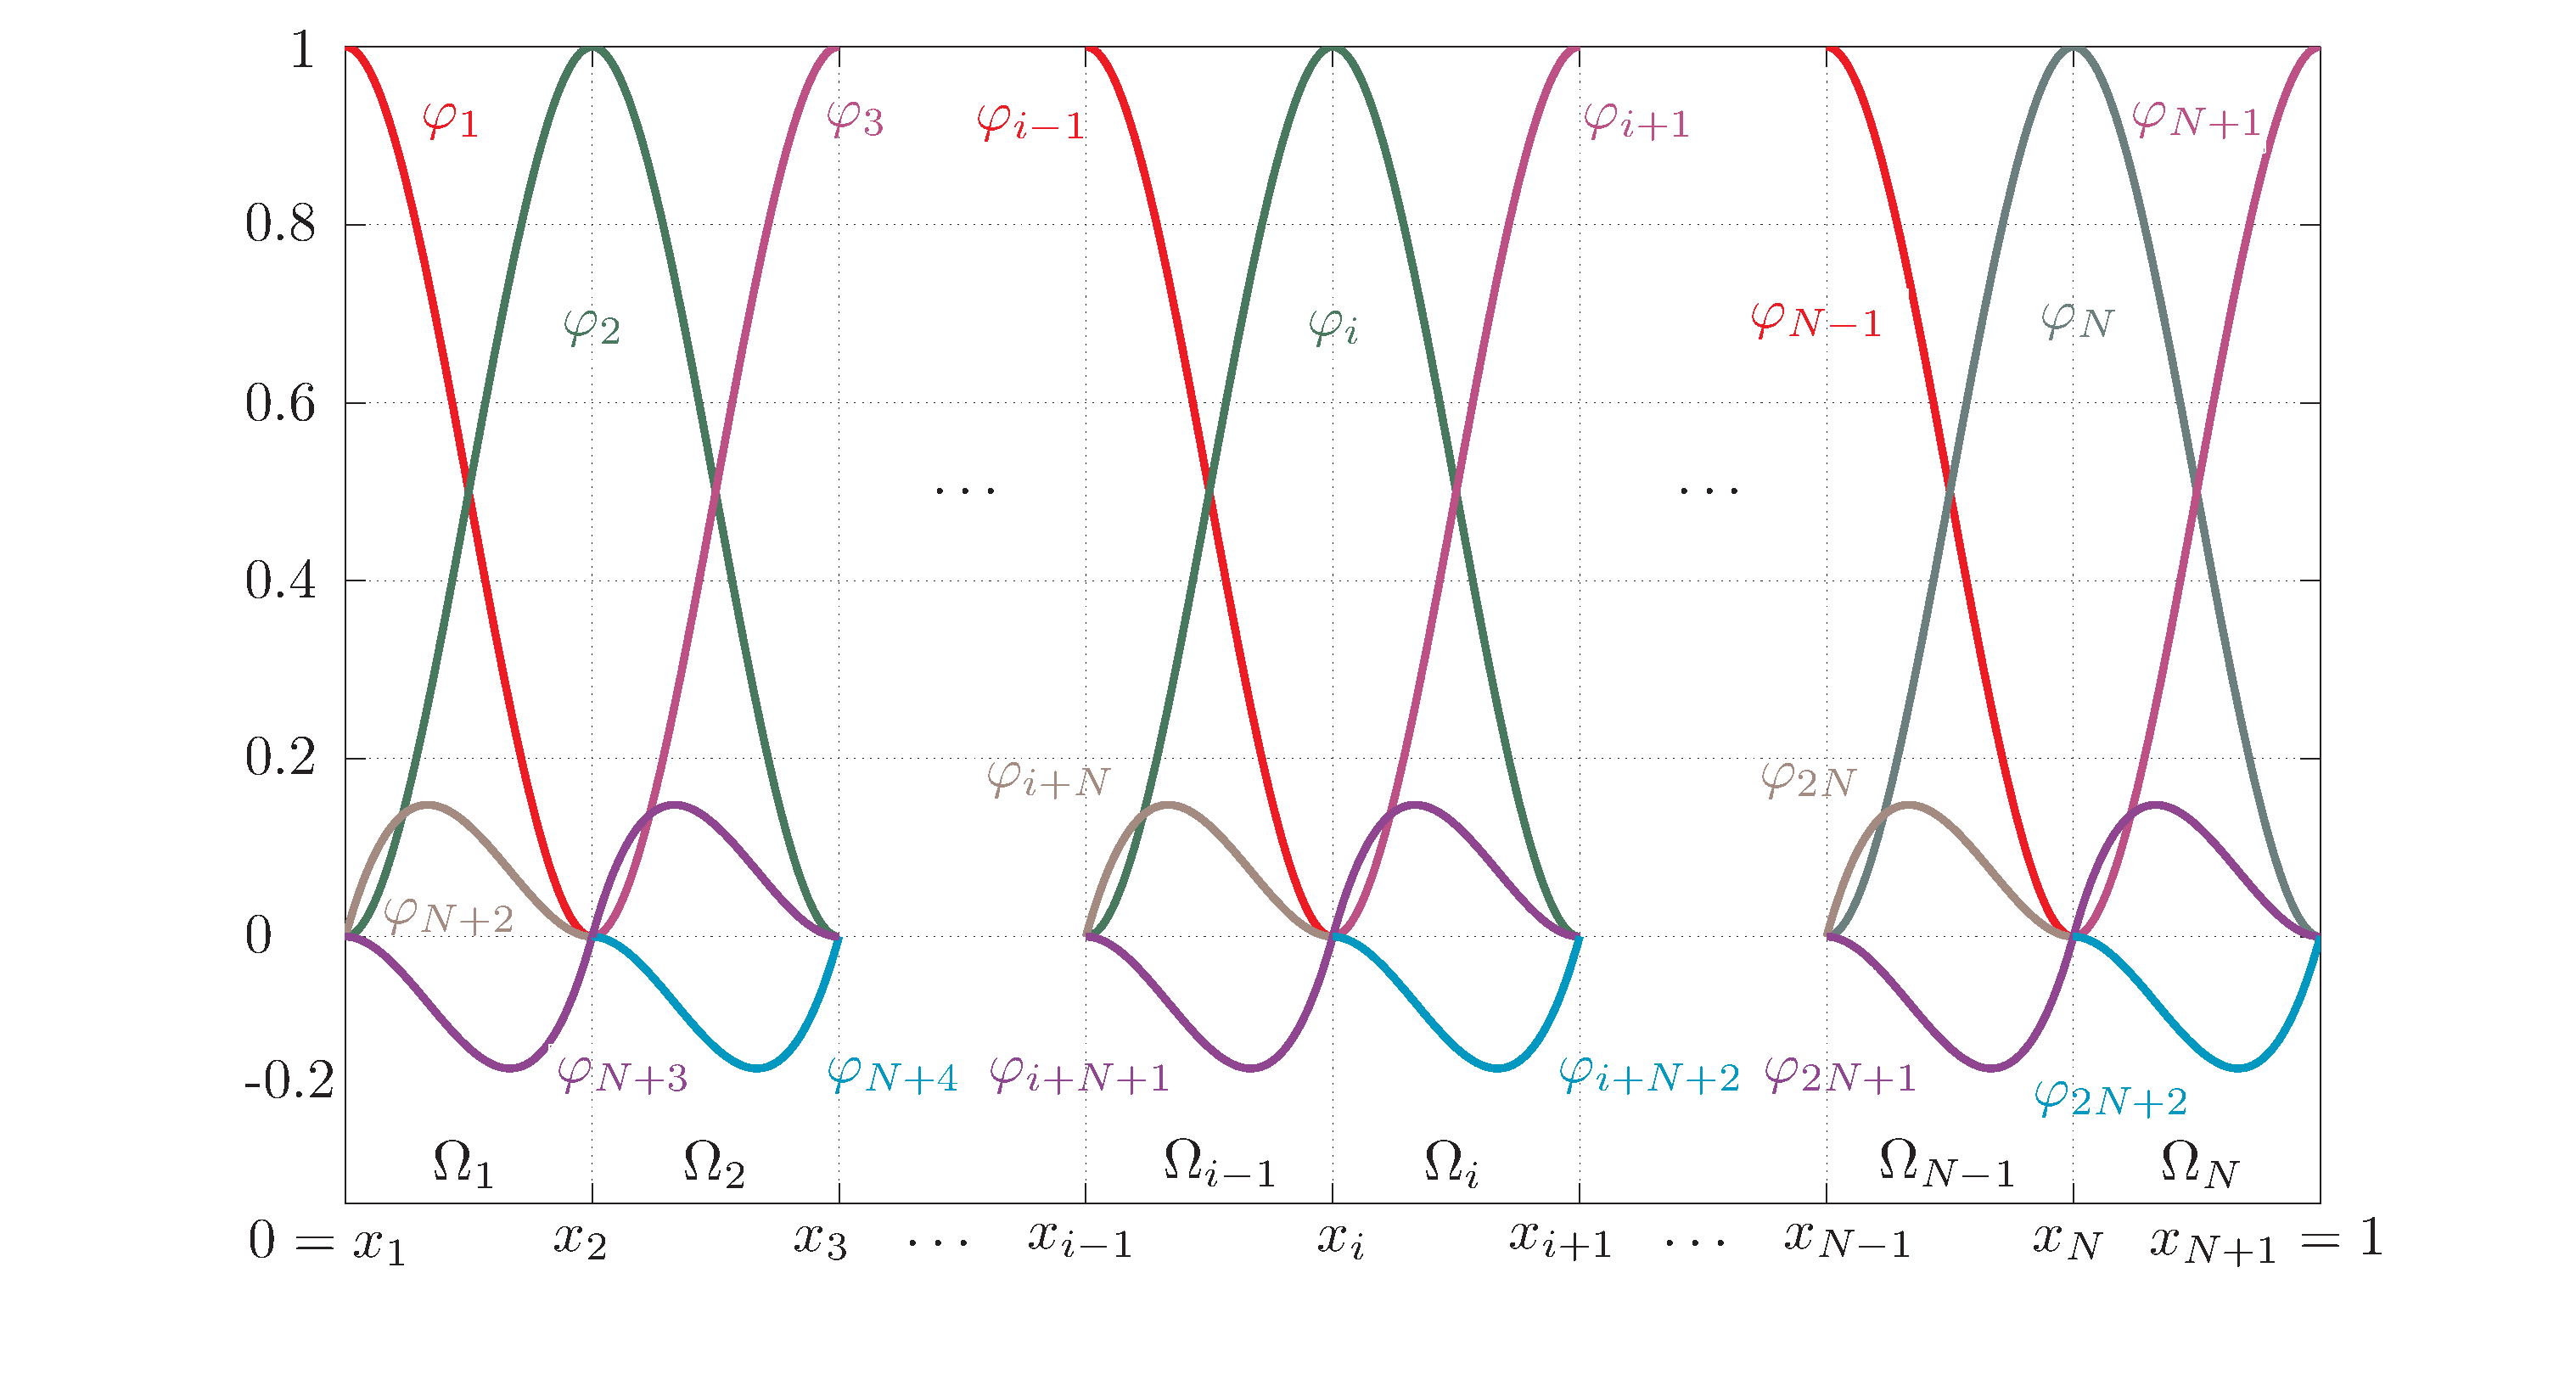
\includegraphics[width = \textwidth]{../figures/cubic-basis-functions}
	\caption[Choice of Cubic Polynomials for Basis-Functions]
		{Choice of cubic polynomials for Basis-Functions gives a solution which is $\mathcal{O} \left( 1 \right)$-continuous.}
	\label{fig:Cubic_Basis_Functions}
\end{figure}
%
\subsection[Element Matrix and Element Load]{\Gls{elementMatrix} and \Gls{elementLoad}} \label{cha:Element_Matrix_Load_Cubic}
Above we saw how we could calculate the global \gls{stiffnessMatrix} and \gls{loadVector} by summing element contributions,
see under \cref{cha:Element_Matrix_Linear,cha:Element_Load_Linear,cha:Assembly_Process_Linear}. Note that we defined
two \glspl{shapeFunction} over a typical \gls{element} in the linear case. The \gls{elementMatrix} and \gls{loadVector} for
\gls{linearFEMSol} are then \gls{Ke} $\in$ \glsentryname{R22} and \gls{be} $\in$ \glsentryname{R21}, respectively. In the cubic
case, on the other hand, there are $4$ nonzero \glspl{shapeFunction} over each \gls{element}. Thus
\begin{subequations}
	\begin{alignat}{2}
		\glsentryname{Kmne} &= \frac{1}{h} \int_{0}^{1} q \Bigl[ \left( e - 1 + \xi \right) h \Bigr] \frac{ d \psi_m }{ d \xi }
			\frac{ d \psi_n }{ d \xi } \dd \xi,	\quad& m, n = 1, \dots, 4,	\label{eqn:Cubic_Element_Stiffness_Entries}	\\
			b_{m}^{e} &= h \int_{ 0 }^{ 1 } f \biggl[ h \left( e - 1 + \xi \right) \biggr] \psi_m \left( \xi \right) \dd \xi,
				\quad& m = 1, \dots, 4.	\label{eqn:Cubic_Element_Load_Entries}
	\end{alignat}
\end{subequations}	\text{}
\Cref{lst:Elem_Cont} shows MATLAB code for implementation of element contributions in both linear and cubic case.
%
\subsection{Assembly Process} \label{cha:Assembly_Process_Cubic}
Again, denote by \gls{K} and \gls{b} the global \gls{stiffnessMatrix} and \gls{loadVector}. Also let \gls{KGlobalE} and
\gls{bGlobalE} describe status of \gls{K} and \gls{b} after addition of element and load contributions from elements
$1,2, \ldots, e$. Then assembly process with cubic basis functions are visualized in \crefrange{fig:K_1_Cubic}{fig:K_4_Cubic} and \cref{fig:b_1_To_b_4_Cubic}. MATLAB code in \cref{lst:Setup_Eq_Sys} implements this process in both linear and cubic case.

% ------------------ Insert Visualization of Cubic Assembly Process ------------------
% Cubic K^{1}
\begin{sidewaysfigure}[H]
	\centering
	\begin{equation*}
		\mathbf{K}^{\left( 1 \right)} =
		\begin{bmatrix}
			k_{11}^{1} & k_{12}^{1} & 0 & 0 & 0 & k_{13}^{1} & k_{14}^{1} & 0 & 0 & 0 \\ \\
			k_{21}^{1} & k_{22}^{1} & 0 & 0 & 0 & k_{23}^{1} & k_{24}^{1} & 0 & 0 & 0 \\ \\
			0 & 0 & 0 & 0 & 0 & 0 & 0 & 0 & 0 & 0 \\ \\
			0 & 0 & 0 & 0 & 0 & 0 & 0 & 0 & 0 & 0 \\ \\
			0 & 0 & 0 & 0 & 0 & 0 & 0 & 0 & 0 & 0 \\ \\
			k_{31}^{1} & k_{32}^{1} & 0 & 0 & 0 & k_{33}^{1} & k_{34}^{1} & 0 & 0 & 0 \\ \\
			k_{41}^{1} & k_{42}^{1} & 0 & 0 & 0 & k_{43}^{1} & k_{44}^{1} & 0 & 0 & 0 \\ \\
			0 & 0 & 0 & 0 & 0 & 0 & 0 & 0 & 0 & 0 \\ \\
			0 & 0 & 0 & 0 & 0 & 0 & 0 & 0 & 0 & 0 \\ \\
			0 & 0 & 0 & 0 & 0 & 0 & 0 & 0 & 0 & 0
			\end{bmatrix}
	\end{equation*}
	\caption{Stiffness Assembly with Cubic Basis-Functions, $\mathbf{K}^{\left( 1 \right)}$}
	\label{fig:K_1_Cubic}	
\end{sidewaysfigure}
%
% Cubic K^{2}
\begin{sidewaysfigure}[H]
	\centering
	\begin{equation*}
		\mathbf{K}^{\left( 2 \right)} =
		\begin{bmatrix}
			% 1. row
			k_{11}^{1} & k_{12}^{1} & 0 & 0	& 0 & k_{13}^{1} & k_{14}^{1} & 0 & 0 & 0 \\ \\
			% 2. row
			k_{21}^{1}&k_{22}^{1}+k_{11}^{2}&k_{12}^{2}&0 & 0 & k_{23}^{1} & k_{24}^{1}+k_{13}^{2} & k_{14}^{2} & 0 & 0 \\ \\
			% 3. row
			0 & k_{21}^{2} & k_{22}^{2} & 0 & 0 & 0 & k_{23}^{2} & k_{24}^{2} & 0 & 0 \\ \\
			% 4. row
			0 & 0 & 0 & 0 & 0 & 0 & 0 & 0 & 0 & 0 \\ \\
			% 5. row
			0 & 0 & 0 & 0 & 0 & 0 & 0 & 0 & 0 & 0 \\ \\
			% 6. row
			k_{31}^{1} & k_{32}^{1} & 0 & 0 & 0 & k_{33}^{1} & k_{34}^{1} & 0 & 0 & 0 \\ \\
			% 7. row
			k_{41}^{1}&k_{42}^{1}+k_{31}^{2}&k_{32}^{2}&0& 0 & k_{43}^{1} & k_{44}^{1}+k_{33}^{2} & k_{34}^{2} & 0 & 0 \\ \\
			% 8. row
			0 & k_{41}^{2} & k_{42}^{2} & 0 & 0	& k_{43}^{2} & k_{44}^{2} & 0 & 0 & 0 \\ \\
			% 9. row
			0 & 0 & 0 & 0 & 0 & 0 & 0 & 0 & 0 & 0 \\ \\
			% 10. row
			0 & 0 & 0 & 0 & 0 & 0 & 0 & 0 & 0 & 0
		\end{bmatrix}
	\end{equation*}
	\caption{Stiffness Assembly with Cubic Basis-Functions, $\mathbf{K}^{\left( 2 \right)}$}
	\label{fig:K_2_Cubic}
\end{sidewaysfigure}
%
% Cubic K^{3}
\begin{sidewaysfigure}[H]
	\centering
	\begin{equation*}
		\mathbf{K}^{\left( 3 \right)} =
		\begin{bmatrix}
			% 1. row
			k_{11}^{1} & k_{12}^{1} & 0 & 0 & 0 & k_{13}^{1} & k_{14}^{1} & 0 & 0 & 0 \\ \\
			% 2. row
			k_{21}^{1} & k_{22}^{1}+k_{11}^{2} & k_{12}^{2} & 0 & 0 & k_{23}^{1} & k_{24}^{1}+k_{13}^{2} & k_{14}^{2} & 0 & 0 \\ \\
			% 3. row
			0 & k_{21}^{2} & k_{22}^{2}+k_{11}^{3} & k_{12}^{3} & 0 & 0 & k_{23}^{2} & k_{24}^{2}+k_{13}^{3} & k_{14}^{3} & 0 \\ \\
			% 4. row
			0 & 0 & k_{21}^{3} & k_{22}^{3} & 0 & 0 & 0 & k_{23}^{3} & k_{24}^{3} & 0 \\ \\
			% 5. row
			0 & 0 & 0 & 0 & 0 & 0 & 0 & 0 & 0 & 0 \\ \\
			% 6. row
			k_{31}^{1} & k_{32}^{1} & 0 & 0 & 0 & k_{33}^{1} & k_{34}^{1} & 0 & 0 & 0 \\ \\
			% 7. row
			k_{41}^{1} & k_{42}^{1}+k_{31}^{2} & k_{32}^{2} & 0 & 0 & k_{43}^{1} & k_{44}^{1}+k_{33}^{2} & k_{34}^{2} & 0 & 0 \\ \\
			% 8. row
			0 & k_{41}^{2} & k_{42}^{2}+k_{31}^{3} & k_{32}^{3} & 0 & 0 & k_{43}^{2} & k_{44}^{2}+k_{33}^{3} & k_{34}^{3} & 0 \\ \\
			% 9. row
			0 & 0 & k_{41}^{3} & k_{42}^{3} & 0 & 0 & 0 & k_{43}^{3} & k_{44}^{3} & 0 \\ \\
			% 10. row
			0 & 0 & 0 & 0 & 0 & 0 & 0 & 0 & 0 & 0
		\end{bmatrix}
	\end{equation*}
	\caption{Stiffness Assembly with Cubic Basis-Functions, $\mathbf{K}^{\left( 3 \right)}$}
	\label{fig:K_3_Cubic}
\end{sidewaysfigure}
%
% Cubic K^{4}
\begin{sidewaysfigure}[H]
	\centering
	\begin{equation*}
		\mathbf{K}^{\left( 4 \right)} =
		\begin{bmatrix}
			% 1. row 
			k_{11}^{1} & k_{12}^{1}	& 0	& 0 & 0 & k_{13}^{1} & k_{14}^{1} & 0 & 0 & 0 \\ \\
			% 2. row
			k_{21}^{1}&k_{22}^{1}+k_{11}^{2} & k_{12}^{2} & 0 & 0 & k_{23}^{1} & k_{24}^{1}+k_{13}^{2} & k_{14}^{2} & 0 & 0 \\ \\
			% 3. row
			0&k_{21}^{2} & k_{22}^{2}+k_{11}^{3} & k_{12}^{3} & 0 & 0 & k_{23}^{2} & k_{24}^{2}+k_{13}^{3} & k_{14}^{3} & 0 \\ \\
			% 4. row
			0 & 0 & k_{21}^{3} & k_{22}^{3}+k_{11}^{4} & k_{12}^{4} & 0 & 0 & k_{23}^{3} & k_{24}^{3}+k_{13}^{4} & k_{14}^{4} \\ \\
			% 5. row
			0 & 0 & 0 & k_{21}^{4} & k_{22}^{4} & 0 & 0 & 0 & k_{23}^{4} & k_{24}^{4} \\ \\
			% 6. row
			k_{31}^{1} & k_{32}^{1} & 0 & 0 & 0 & k_{33}^{1} & k_{34}^{1} & 0 & 0 & 0 \\ \\
			% 7. row
			k_{41}^{1}&k_{42}^{1}+k_{31}^{2} & k_{32}^{2} & 0 & 0 & k_{43}^{1} & k_{44}^{1}+k_{33}^{2} & k_{34}^{2} & 0 & 0 \\ \\
			% 8. row
			0&k_{41}^{2} & k_{42}^{2}+k_{31}^{3} & k_{32}^{3} & 0 & 0 & k_{43}^{2} & k_{44}^{2}+k_{33}^{3} & k_{34}^{3} & 0 \\ \\
			% 9. row
			0 & 0 & k_{41}^{3} & k_{42}^{3} + k_{31}^{4} & 0 & 0 & 0 & k_{43}^{3} & k_{44}^{3} + k_{33}^{4} & k_{34}^{4} \\ \\
			% 10. row
			0 & 0 & 0 & k_{41}^{4} & k_{42}^{4} & 0 & 0 & 0 & k_{43}^{4} & k_{44}^{4}
		\end{bmatrix}
	\end{equation*}
	\caption{Stiffness Assembly with Cubic Basis-Functions, $\mathbf{K}^{\left(4\right)}$ }	
	\label{fig:K_4_Cubic}
\end{sidewaysfigure}
%
% Insert Cubic Load Assemby figure here
\begin{figure}[H]
	\centering
	\begin{equation*}
	\begin{aligned}
	% b_{1}
	\mathbf{b}^{\left( 1 \right)} &=
	\begin{bmatrix}
	b_{1}^{1} & b_{2}^{1} & 0 & 0 & 0 & b_{3}^{1} & b_{4}^{1} & 0 & 0 & 0
	\end{bmatrix}^{T},	\\
	% b_{2}
	\mathbf{b}^{\left( 2 \right)} &=
	\begin{bmatrix}
	b_{1}^{1} & b_{2}^{1} + b_{1}^{2} & b_{2}^{2} & 0 & 0 & b_{3}^{1} & b_{4}^{1} + b_{3}^{2} & b_{4}^{2} & 0 & 0
	\end{bmatrix}^{T},	\\
	% b_{3}
	\mathbf{b}^{\left( 3 \right)} &=
	\begin{bmatrix}
	b_{1}^{1} & b_{2}^{1} + b_{1}^{2} & b_{2}^{2} + b_{1}^{3} & b_{2}^{3} & 0 & b_{3}^{1} & b_{4}^{1} + b_{3}^{2} &
	b_{4}^{2} + b_{3}^{3} & b_{4}^{3} & 0
	\end{bmatrix}^T,	\\
	% b_{4}
	\mathbf{b}^{\left( 4 \right)} &=
	\begin{bmatrix}
	b_{1}^{1} & b_{2}^{1} + b_{1}^{2} & b_{2}^{2} + b_{1}^{3} & b_{2}^{3} + b_{1}^{4} & b_{2}^{4} & b_{3}^{1} &
	b_{4}^{1} + b_{3}^{2} & b_{4}^{2} + b_{3}^{3} & b_{4}^{3} + b_{3}^{4} & b_{4}^{4}
	\end{bmatrix}^{T}.
	\end{aligned}
	\end{equation*}
	\caption{Load Assembly with Cubic Basis-Functions, $\mathbf{b}^{\left(1\right)}, \dots, \mathbf{b}^{\left(4\right)}$}
	\label{fig:b_1_To_b_4_Cubic}
\end{figure}
%
%
Another way of explaining the assembly process follows:
\begin{enumerate}
	\item For each element $e$ calculate \gls{Ke} and \gls{be} from
	\cref{eqn:Cubic_Element_Stiffness_Entries,eqn:Cubic_Element_Load_Entries}.

	\item \Gls{elementMatrix} \gls{Ke} $\in$ \glsentryname{R44} may then be divided into $4$ sub-matrices all of them in \glsentryname{R22} i.e., upper/lower left and right. Add these sub-matrices to the global \gls{stiffnessMatrix} entries
	starting at entries $K_{e, e}$, $K_{e + N + 1, e}$, $K_{e, e + N + 1}$ and $K_{e + N + 1,e + N + 1}$, respectively.

	\item \Gls{elementLoad} \gls{be} $\in$ \glsentryname{R41}, on the other hand, is divided to two sub vectors of size
	$2\times 1$ each, i.e., upper and lower. These sub vectors are then added to the global \gls{loadVector} starting at entries
	$b_{e}$ and $b_{e + N + 1}$, respectively.
\end{enumerate}
%
\subsection[Implementation of Boundary Conditions]{Implementation of \glspl{boundaryCondition}}
The essential condition $u(0)=\delta$ is imposed directly on the left endpoint value degree of freedom. The natural condition in \cref{eqn:FEM_Right_Boundary} enters through the boundary functional $P w(1)$ in \cref{eqn:Weak_Formulation}. Consequently, $P$ is added to the equation associated with the right endpoint value for both the linear and cubic systems.

The cubic basis also contains a right endpoint slope degree of freedom. Its basis function has zero value at $x=1$, so the natural boundary functional contributes nothing to that equation. The slope equation therefore remains part of the assembled Galerkin system; prescribing the slope separately would overconstrain the discrete problem. \emph{MATLAB} code in \cref{lst:Solve_Eq_Sys} implements this treatment.
%

\section{Buildup finite element solution}
The next step is to solve this system and find the unknowns. This is done by using \emph{MATLAB Equation Solver}. For large No.
of elements we should take advantage of the sparse system property to save both memory and processor resources. This means that
we don't have to save the full stiffness matrix and \gls{loadVector}, but just nonzero diagonals in \gls{stiffnessMatrix} and load vector.
For the \gls{sparseMat} we also have access to much more efficient solver \glspl{algorithm}. For the problem in hand,
however, we have saved and solved the full system. \Cref{lst:Build_Sol} shows the MATLAB code for building up \gls{FEMSol} with
both linear and cubic \glspl{basisFunction}.
\begin{remark}
	The primary solution in some numerical methods\footnote{Such as \glspl{finiteDiffMethod}.} are the function values at
	predefined nodal points. In each case a smooth solution may then be constructed by interpolating these points. In FEM, on the
	other hand, interpolation is an integrated part of the method, see \cref{eqn:Truncated_FEM_Solution}.
\end{remark}	\text{}
For a discussion of these and other relevant materials consult \cite{Bertoti:1997,Carlson:1967,KarelRektorys:1975,Szeidl:2001}.
